\documentclass[11pt,letter]{article}
\usepackage[top=0.50in, bottom=0.7in, left=1.1in, right=1.1in]{geometry}
\usepackage{graphicx} % Required for inserting images
\usepackage{xcolor} 
\definecolor{Accent}{HTML}{bd2b00} 
\usepackage[numbers,compress,super]{natbib}
\usepackage{gensymb}
\usepackage{hyperref}
\hypersetup{colorlinks,citecolor = Accent, linkcolor = Accent,urlcolor = Accent, breaklinks=true}
\usepackage{cleveref}
\usepackage[labelfont=bf]{caption}
\bibliographystyle{unsrtnat}

\RequirePackage[labelfont={bf,sf},%
                font={small, sf}]{caption}

\usepackage{lineno}
\renewcommand\linenumberfont{\normalfont\tiny\color{gray}}

\begin{document}

\title{Overlooked model uncertainties may misinform forest management strategies}

\author{Victor, Jérôme, Isabelle} % and more?
\date{}
\maketitle 


\noindent\rule{\textwidth}{0.3pt}
\textbf{Abstract---still need work:} Forests play a major role in mitigating climate change, but increasing threats to forests from climate change have heightened the importance of managing these systems. Robust forecasts of forest composition with increasing climate change are critical to this aim, but are currently highly variable. To help guide management in the face of this variability and understand where we can most rapidly reduce uncertainty through improved models, we compare over 1350 ecological models and climate scenarios in forecasts for forests across Europe. Our approach considers a gradient of more mechanistic (`process-based') to correlative models of species distributions to find that uncertainty in ecological models can drive more variation than vastly different climate scenarios (e.g., SSP2 vs. SSP5), but also areas with relatively consistent projections [give overview of these and say that this could reduce uncertainty in how to manage for these areas]. [Maybe something on using existing range data leads to more pessimistic forecasts?] Our results highlight a new way to approach ecological forecasting that better identifies areas of higher certainty and, conversely, the areas where managers will need more diversified approaches and where more ecological study may be most useful.

\noindent\rule{\textwidth}{0.3pt}

\linenumbers

\subsection*{Main}
%
%Intro:
%1. Basically first two paragraphs you have combined (we need forests to
%store C, and they are doing poorly) ending on the need for better
%guidance of forest management
%2. This is hard because we have a lot of biological models and they give
%different answers, and for management we need to layer on the future
%climate models ...
%- Go into briefly the correlative versus process models -- they
%differ  but we're not sure which is best
%- Given we don't have one great approach to build to (and we have
%run out of time), so maybe we move on and accept the diversity
%- Transition to something explaining the layers of models we need
%to consider to capture climate to biology
%3. Back to what we need to do with the models for forest management
%- Here you might touch on what we could do with this, get in some
%of the stuff I highlighted in the discussion that you need to foreshadow
%for readers.


%From J Chave:
%Climate change has direct impact on a myriad of ecosystem processes, and forests are especially vulnerable. European temperatures are rising twice as fast as the global average (Copernicus Climate Change Service, 2024), and unprecedented pulses of tree mortality have benn reported in the last decade, across the range of forest species (Senf et al, 2020). As a consequence, some European forests are now net CO2 sources (Hadden and Grelle, 2016; Karelin et al, 2021), due to decreased growth (Hadden and Grelle, 2016; van der Woude et al, 2023), increased burned areas (Carnicer et al, 2022; Kelly et al, 2024), and increased pest or drought-related dieback driven (Cienciala and Melichar, 2024; Karelin et al, 2021; Latifovic and Arain, 2024).  Implementation strategies are rolled out in spite of the uncertainty of the scenarios.

%1. Basically first two paragraphs you have combined (we need forests to
%store C, and they are doing poorly) ending on the need for better
%guidance of forest management
% the baby: with climate change, we need to safeguard and adapt forests, as they play a major role in mitigating its effects
Forests are key to pursuing climate change mitigation policies and achieving carbon neutrality  \citep{Korosuo2023, Hyyrynen2023}. Yet, forests are increasingly under pressure. In Europe, temperatures are rising twice as fast as the global average \citep{CCCS2024}, and unprecedented pulses of tree mortality  have been reported in the last decade \citep{Senf2020}. As a result, some European forests are becoming net CO$_2$ sources \citep{Hadden2016, Karelin2021}, due to decreased growth \citep{Hadden2016, Woude2023}, larger burned areas \citep{Carnicer2022, Kelly2024}, and increased pest- and drought-induced dieback \citep{Karelin2021, Cienciala2024, Latifovic2024}. Forest managers are facing unprecedented challenges, as they must address current threats while also promoting long-term adaptation to climate change. In this context of high uncertainty, better guidance  is needed to implement successful strategies.
% and evidence-based projections are

%2. This is hard because we have a lot of biological models and they give
%different answers, and for management we need to layer on the future
%climate models ...
%- Go into briefly the correlative versus process models -- they
%differ  but we're not sure which is best
%- Given we don't have one great approach to build to (and we have
%run out of time), so maybe we move on and accept the diversity
%- Transition to something explaining the layers of models we need
% the werewolf: We have many models, we don't know which one is the best. Most decisions rely on limited models without much insight into what drives differences in projections. This can mask significant uncertainties and ultimately threaten the success of forest management decisions
% the silver bullet: accept a greater diversity of models (scientific approaches, hypothesis), and figure out how to safeguard forests by gaining a better understanding of uncertainties, i.e., merging across biological and climatological components (uncertainty budget framework)
Given the diversity of predictive ecological models, the challenge of providing practical insights for forest management is even greater. Different models, ranging from correlative to more mechanistic approaches, may provide highly divergent projections \citep{Morin2009, Keenan2011a, Cheaib2012, Takolander2019}. While it remains unclear under which conditions one approach is more reliable than another \citep{VanderMeersch2024}, most projections still rely on a limited set of models \citep{Dyderski2018, Wessely2024, Hanewinkel2013, Schueler2014}, ultimately increasing the risk of policy and management failures \citep{Dawson2011}. We often lack a robust estimation of uncertainty and a comprehensive understanding of what drives differences between projections \citep{Simmonds2024}. Given the urgency of climate change, we must incorporate the diversity of models and merge across ecological and climatological models to provide a complete picture of both the threats and opportunities for forests. 

%3. Back to what we need to do with the models for forest management
%- Here you might touch on what we could do with this, get in some
%of the stuff I highlighted in the discussion that you need to foreshadow
%for readers.
Gaining a better understanding of where uncertainties originate and how they relate is crucial to identify opportunities 
% for model developments \citep{Petchey2015} and  % maybe off-topic? keep for discussion?
to address policy-relevant questions \citep{Urban2016, Saltelli2020, Johnson2024}. Species shifts are predicted to have major impacts on timber production and on the forest economic sector \citep{Wessely2024, Hanewinkel2013}. Forest managers need to know whether the current species will be able to tolerate future climate conditions, whether they can rely on its natural regeneration, or whether they should capitalize on new species opportunities. If the main driver of variation across projections is the different ecological models, even more than different global emissions scenarios, it becomes critical to encompass the a wide range of models. Failing to do so could lead to overly confident predictions about which species will or will not be able to survive in future climates, ultimately leading to counterproductive or even detrimental forest management decisions.

To understand the level of confidence we can place in predictions requires a framework that account for all the various components of climatological and biological uncertainties, including socioeconomic scenarios, global climate models, ecological models, down to the species level. To this aim, we combined over 1350 projections of forest tree species distributions, incorporating a wide range of models, from more mechanistic (‘process-based’) to correlative models. Fully accounting for our current level of knowledge about future climate states and species functioning allows us to quantify the contribution of each component to the total variation across projections. This approach represents a significant advancement over previous studies, which overlooked large portions of uncertainty, and will lead to better informed decision-making to improve the resilience of forests.

% Note: what should be in the intro:
% huge differences between projections, more importanmt than species or SSP, toget a comprehensive assesment of the magnitude of climatic change?
%  ignoring a large portion of uncertainty in psecies range projections due to modelling approaches can thus lead to baaad decisions.


\begin{figure}
	\centering
	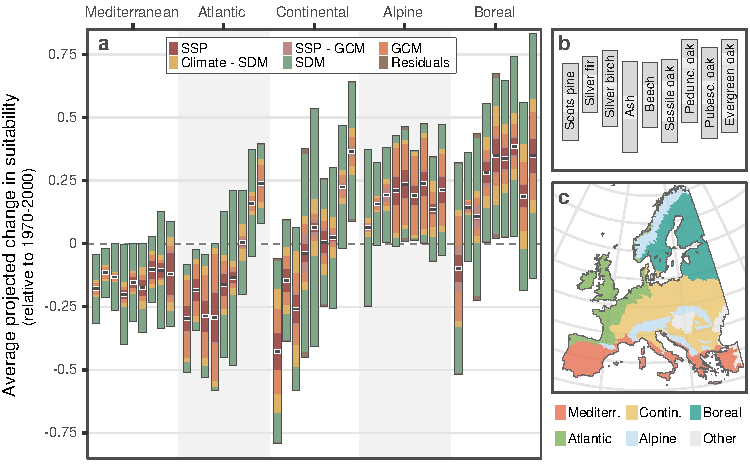
\includegraphics[width=0.85\linewidth]{../newfigures/files/figure1}
	\caption{\textbf{Ecological models represent the main source of uncertainty in future projections of species climatic suitability across European biomes (2080-2100)}.}
	\label{fig:anovaspecies}
\end{figure}

\subsection*{Results and discussion}

Our dataset included 9 tree species, both deciduous and coniferous, adapted to diverse climatic conditions across Europe. We simulated their suitability from 1970 to 2100, at a 0.1\degree~spatial resolution, using a diverse set of ecological models spanning different hypotheses and calibration methods. We used 10 different future climate simulations, based on 2 forcing scenarios and 5 global climate models with different climate sensitivities.

% uncertainty in ecological models can drive more variation than vastly different climate scenarios 
Across species, ecological models drive more variation than vastly different climate scenarios (\Cref{fig:anovaspecies}). They consistently represent the main source of uncertainty across major European biomes (explaining between 42.9\% and 63.9\% of the variation between projections), with the exception of the Alpine biome. At the species-level, across all biomes, the differences between ecological models is also the main source of uncertainty for all the species considered here, and represents between 40\% and 62\% of the total uncertainty on average. One of the striking example is the climatic suitability change of sessile oak in the Atlantic region, where this species represents an important cultural and economic value, and for which more than 80\% of the uncertainty in climate change impact projections was due to variations among ecological models. 

% The differences among climate model projections (GCMs) and socioeconomic scenarios (SSPs). 
% in the Continental ecoregion, differences across models account for 73.7% of the total uncertainty of beech future suitability, despite being within the core of its present distribution. Similarly, SDM is the main source of uncertainty for sessile and pedunculate oaks (respectively 57% and 76.8%, Figure 22).

Failing to account for a broad range of ecological models severely underestimate projection uncertainty, and ultimately lead to incorrect trend estimates (\Cref{fig:cascade}). Considering only correlative models would have misled to an overestimation of the contribution of climate projections (forcing scenarios, climate models, and their two-way interaction) to the total projection uncertainty in all regions, except the Mediterranean. In particular, divergence between climate models would have appeared to contribute as much as ecological models to projection uncertainty (on average, 36.6\% and 37.5\%, respectively). When accounting for more diverse ecological models, as done in our study, the uncertainty introduced by different ecological models (51.0\% on average for all species) becomes greater than that introduced by climate models (19.9\%). One of the key challenges for reducing uncertainty thus remains at the biological and ecological levels, even before considering the broad variations across future climate projections.
% At biome scale: e.g. continental: 54.3% of SDM with full diveristy (GCM: 14.10%), only 27.95% when considering only correlative models (46.22% for GCM)
% Also true a the species-level: SDM 50.77 down to 27.46, GCM 15.85 up to 35.95%

% For example, for beech, we would have estimated that discrepancies between GCMs would have been the major source of uncertainties (39.8\%), higher than the SDM uncertainty (33.8\%), whereas it was in reality much lower (18.8\%) than SDM uncertainty (51.2\%) when considering the three approaches of SDMs. Ignoring a large portion of uncertainty in species range projections due to modelling approaches can thus lead to overly confident predictions about which species will or will not be able to survive in future climates.  This becomes increasingly true as we approach the end of the 21\textsuperscript{st} century, where larger climate changes result in larger variation among projections (\Cref{fig:anovaecoregions}).
% there is a strong interest in considering a broader range of models to better characterize projections uncertainty.

\begin{figure}
	\centering
	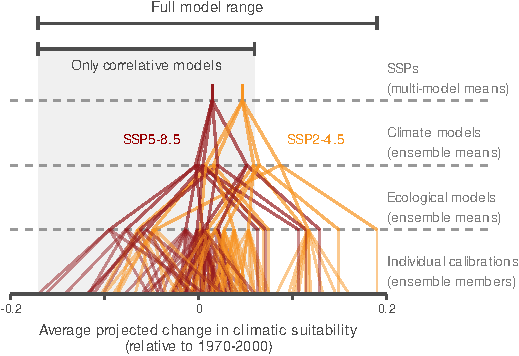
\includegraphics[width=0.6\linewidth]{../newfigures/files/uncertaintycascade}
	\caption{\textbf{Considering a broad range of models provides a more comprehensive view of possible future scenarios.}}
	\label{fig:cascade}
\end{figure}

% [Maybe something on using existing range data leads to more pessimistic forecasts?]
Our results also revealed that the divergence between ecological model projections followed a regular pattern. Models calibrated using current species range data consistently predict greater extinctions than models calibrated using experimental data (\Cref{fig:diffproj}). 
%Especially in Mediterranean and Atlantic ecoregions and in the western part of the Continental ecoregion (Figures 23). Overall, expert PEMs also simulated a higher increase of suitability in the transition zone between Continental and Boreal ecosystems. Fitted PEMs
Current distribution data may capture only a portion of the climatic niche of a species, underestimating the range of conditions where it could survive \citep{Chevalier2024, NoguesBravo2016}.
% do not account for the physiological processes behind species distribution
These discrepancies between models can significantly alter country-level projections, and impact national strategies derived from them. 
For example, by the end of the 21st century, beech showed an average suitability decrease of -0.19 ($\pm$0.14) across its historical distribution when considering only models entirely calibrated with current species distribution data, leading to an average loss of 30.5\% of its historical distribution (\Cref{fig:diffproj}). But this decreasing trend vanish once a broad range of models is accounted for (-0.028 $\pm$0.17).
Relying on a narrow set of models---especially derived from the same calibration process---undermines the robustness of projections \citep{Dawson2011}, and may ultimately bias decisions towards intensive intervention strategies (e.g. introduction of species outside their native range), potentially overlooking alternative strategies.
% Multi-model ensembles have been so far mostly restricted to statistical models (Simmonds et al, 2024), but we show here that there is a strong interest in considering a broader range of models to better characterize projections uncertainty. 


% \item which implications in terms  of forest management? 
%\begin{enumerate}
%	\item on average, uncertain projections = more possibilities to act? more adaptation measures
%	\item but high uncertainties may lead to \emph{laissez-faire}
%	\item we want to avoid that, how to translate uncertainties into decision-making?\\
%	$\rightarrow$ favor forest adaptation strategies resilient to a wide range of possible future conditions.
%	\item forest managers, policy makers:\\
%	rethink the way species distribution modeling is applied to forest management\\
%\end{enumerate}

\begin{figure}
	\centering
	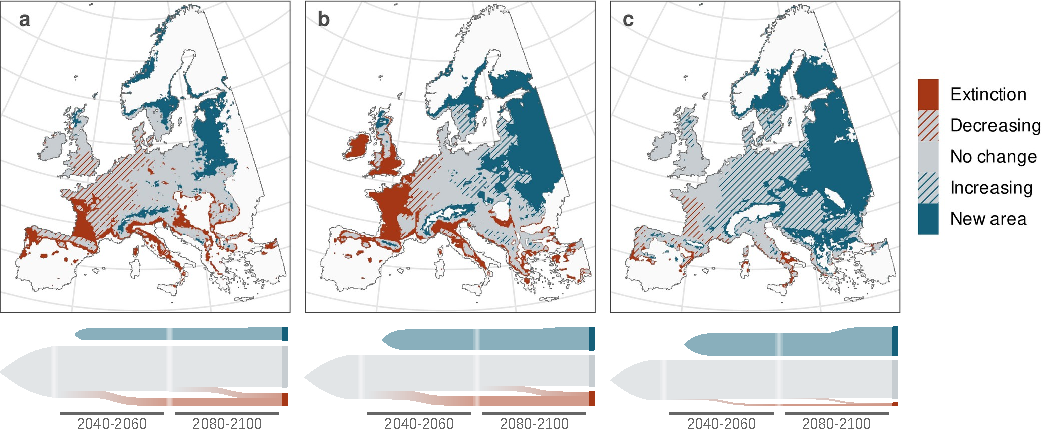
\includegraphics[width=1\linewidth]{../newfigures/files/sankey/fagus_sankey.pdf}
	\caption{\textbf{Models build on current species range data project higher extinctions.}}
	\label{fig:diffproj}
\end{figure}

% this paragraph is not very exciting, its feels like a looong list ("un inventaire à la Prévert")
Despite large uncertainties, comparing diverse models improve prediction robustness and enable to identify areas with relatively consistent projections that differ in terms of future climate risks and levers of action to address them (\Cref{fig:manag}).
Around the Mediterranean Basin, the models consistently predict less favorable climatic conditions for the species we considered here. In areas where most species are threatened, forest managers may thus consider introducing more drought-tolerant species. Along the Atlantic margin, the suitability of most species is also projected to decrease, except for the two Mediterranean species---pubescent and evergreen oaks--- which could replace less adapted temperate species such as beech \citep{Penuelas2003}. Mechanistic model projections are less pessimistic for deciduous oaks and beech (\Cref{fig:diffproj}), suggesting that some better-adapted populations could survive if the existing standing genetic variation is maintained and promoted by forest managers \citep{Brang2014}. Additionally, adapting management practices, such as decreasing stand density to limit competition for water, could support their long-term survival to drought events \citep{Young2023}.\\
A large part of the Continental biome exhibit less clearer trends (\Cref{fig:manag}), as well as mountainous regions at the transition between Mediterranean and Continental/Atlantic climates (Pyrenees, Massif Central, Balkans). Yet, looking at divergence across projections still provide important insights into species and locations most likely to experience significant changes in future climatic conditions. Models agree on a lower suitability for Scots pines (with uncertainty driven more by climatic models and scenarios, 45.7\%, than by ecological models, 30.8\%), which is a commercially very important species [cite] in several countries of Central Europe (such as Poland, Eastern Germany, Czech Republic, Belarus).
Projections also suggest that temperate deciduous species (e.g. beech, deciduous oaks) will be less affected by climate change, despite high uncertainties due to high divergence among ecological models (between 45.7 and 75.4\% of the total uncertainty).
A key lever of action in this region is the diversification of tree species, as well as increasing genetic diversity within populations, to mitigate the risks associated with uncertain future conditions \citep{Morin2014, Ammer2019, Pretzsch2021, Vospernik2024}. Promoting uneven-aged stands could also enhance forest stability by improving structural complexity and buffering against climate extremes \citep{Vangi2024, Zhang2024a}.\\
Finally, boreal biomes in Scandinavian and Baltic countries are projected to get an overall increase of climatic suitability (\Cref{fig:manag}). These include Finland and Sweden, two very important forestry countries in terms of wood stock, added value, and forest-based workforce [cite].
Forests in these regions are dominated by two conifers species, Scots pine and spruce, favoured by commercial forest management. The lack of experimental data prevented us from making mechanistic model projections for spruce, but uncertainty for Scot pine future suitability was very high. Models consistently project that temperate deciduous trees will become more competitive at the northern margin of their range (\Cref{fig:diffproj}), and the extending growing season could offer an opportunity to convert pure coniferous stands into mixed forest to increase their resilience \citep{Schauer2023}.
% idea: Forest management decisions can only be made alongside the development of economic sectors for deciduous species

% Europe: 38.6% forest, and most countries have at least 30% of forest
% Germany account for 13.2% of the stock of timber in the EU's forests 
% Sweden: 12.6% - France : 11.8%, then Poland, Finland Romania, all > 8%
% => these five countries represent more than 50%
%  largest workforce: Sweden, Romania, Germany

% from my PhD discussion:
% As perfectly summarized by \citet{Dawson2011}, "\emph{the heavy reliance of conservation management and policy on a single scientific approach creates risks of policy or management failures, particularly given that the underlying assumptions of that approach are under debate}". Indeed, we have shown that the discrepancies between the different modeling approaches we considered represent a significant share of the uncertainties of future species range shifts (\Cref{fig:cascadebonus}). Researchers may omit some uncertainties because they believe communicating on them can have a negative effect on public trust \citep{Howe2019, Simmonds2024} and may prefer to deliver what they consider a clear message -- sometimes to favor the publication of their results in a competitive academic world \citep{Yao2023}. However, this is a poor strategy because it may decrease public support for science in the long term, particularly if exaggerated pessimistic projections do not ultimately occur \citep{Kreps2020}. Expressing uncertainties may indeed have constructive effects on scientists' credibility, and increase the number of people more supportive of initiatives to tackle climate change \citep{Howe2019}. Importantly, ignoring these uncertainties may also lead to poor management decisions \citep{Simmonds2024}. It could favor intensive intervention strategies (e.g. introduction of species outside their native range), while it might be possible to rather enhance the forest's genetic adaptive capacity. Quantifying and communicating uncertainties -- including by integrating different modeling approaches -- is one of the way to make ecological modeling more relevant to decision making \citep{Dietze2017, Saltelli2020}. 
\clearpage

\begin{figure}
	\centering
	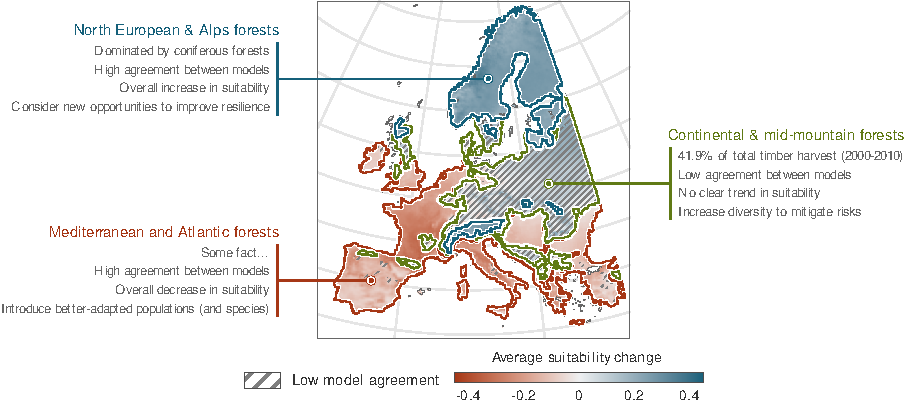
\includegraphics[width=1\linewidth]{../newfigures/files/formanag}
	\caption{\textbf{Accounting for uncertainties supports evidence-based forest management.}}
	\label{fig:manag}
\end{figure}
% conifer-dominated forestry


The implications of these results extend beyond European forests. The large uncertainties we found raise questions about the robustness of existing projections, and highlight that further advances are necessary to provide policy-relevant projections. Given the rapid pace of climate change, there is no time for fruitless debates over which modeling approach to favor. Instead, efforts should focus on bridging diverse methodologies to generate practical insights and support evidence-based decision making. Interdisciplinary synergies will be essential to developing models that are both grounded in mechanistic understanding and statistically robust. Correlative models may be refined by integrating experimental data \citep{Kuo2022}---yet, with some caution \citep{Chevalier2024a}. Mechanistic model improvements should go beyond mere sophistication---adding new processes and new parameters---toward robust statistical inference. Too often, mechanistic models often rely on a single immutable best-parameter set per species \citep{Harrison2021}, preventing any proper propagation of uncertainty. Ultimately, as scientists, we need to be transparent about these uncertainties if we expect forest managers to acknowledge and integrate them \citep{Saltelli2020}. This is the way to make ecological modeling truly relevant to decision making to address complex challenges in a changing climate.



%Looking ahead: a call to action for the scientific community...
%\begin{itemize}
%\item the rapid pace of climate change leaves no time for debates over which modeling approach to favor. Instead, efforts should focus on bridging different methodologies to generate practical insights and support evidence-based decision making.
%\item take advantage of interdisciplinary synergies to build models that are not only grounded in the current mechanistic understanding of the processes but also statistically robust
%\item recent trend to refine correlative models relies on the integration of experimental data \citep{Kuo2022}
%\item mechanistic model refinement should rely not only on sophistication (i.e. adding new processes and parameters)...
%\item we need to go further into uncertainty evaluation, e.g. moving from the \emph{one-unique-parameter-set paradigm} in mechanistic models \citep{Harrison2021}, favor robust inference methods to improve uncertainty propagation
%\item us, as scientists, we need to be transparent about these uncertainties if we want forest managers to tackle them, to include them in the decision making process, i.e. if we want to make ecological modeling more relevant to decision making \citep{Saltelli2020}
%\end{itemize}



%
%	 substantial progress required to develop more reliable projections
%	\item proper evaluation of the transferability?
%  	\item far from l'opposisiton non constructive de differentes ecoles, hypotheses, bridge across to gain practical insights
% M, but also on a step-by-step reassessment and reformulation of the model assumptions, 
%	we have to learn from the different approach, integrate them, of fewer, but more robust models that incorporate mechanistic understanding? simple models can also be great, especially at this scale! considering more diverse data, e.g. phylogeny
% statistical models are evolving towards more mechanistic approaches, 
%	\item going further ? (parameter uncertainty is totally ignored in process-explicit models...), 
%	$\rightarrow$ , i.e; we need to build on similar framework to actually guide adaptation
%\end{enumerate}
% Quantifying and communicating uncertainties -- including by integrating different modeling approaches -- is one of the way to  \citep{Dietze2017, Saltelli2020}. 


\clearpage

\bibliography{phd_bibliography}

\end{document}
